\documentclass[journal,twoside,web]{ieeecolor}
\usepackage{generic}
\usepackage{cite}
\usepackage{amsmath,amssymb,amsfonts}
\usepackage{algorithmic}
\usepackage{graphicx}
\usepackage{algorithm,algorithmic}
\usepackage{hyperref}
\usepackage{textcomp}
\usepackage{url}
\usepackage{makecell}
\usepackage{booktabs}
\usepackage{color}
\usepackage[caption=false,font=footnotesize]{subfig}
\newtheorem{theorem}{Theorem}[section]
\newtheorem{remark}[theorem]{Remark}

\def\BibTeX{{\rm B\kern-.05em{\sc i\kern-.025em b}\kern-.08em
    T\kern-.1667em\lower.7ex\hbox{E}\kern-.125emX}}
\markboth{\hskip25pc IEEE JOURNAL OF BIOMEDICAL AND HEALTH INFORMATICS}
{Author \MakeLowercase{\textit{et al.}}: Title}
\begin{document}
\title{A Risk-Controlled Framework with Guaranteed Confidence for Lung Adenocarcinoma Classification}
\author{Jianxu Wang$^{\dagger}$, Huijun Zhou$^{\dagger}$ and Xuewei Cheng
\thanks{$^{\dagger}$ These authors contributed equally to this work.}
\thanks{This research is supported by the Natural Science Foundation of Hunan Province 2024JJ6303, and the Research Foundation of the Education Department of Hunan Province 23B0056. (Corresponding author: Xuewei Cheng.)}
\thanks{This study involved human participants and was conducted in accordance with the principles of the Declaration of Helsinki. The research protocol entitled “A Risk-Controlled Framework with Guaranteed Confidence for Lung Adenocarcinoma Classification” was reviewed and approved by the Medical Ethics Committee of Hunan Cancer Hospital (approval no. 2026 Scientific Research Expedited Review [106]) on April 22, 2026. The committee granted a final decision of “Approved” under the expedited review procedure. All procedures involving human subjects were performed in compliance with relevant institutional and national regulations.}
\thanks{Jianxu Wang, MOE-LCSM, School of Mathematics and Statistics, Hunan Normal University. E-mail~address: 202330125008@hunnu.edu.cn.}
\thanks{Huijun Zhou, Medical Oncology, Hunan Cancer Hospital. E-mail~address: zhouhuijun@hnca.org.}
\thanks{Xuewei Cheng, MOE-LCSM, School of Mathematics and Statistics, Hunan Normal University; Department of Statistics, University of California, Riverside. E-mail~address: xwcheng@hunnu.edu.cn.}
}

\maketitle

\begin{abstract}
Accurate detection of the micropapillary (MIP) subtype in lung adenocarcinoma is clinically urgent due to its aggressive behavior and poor prognosis. Deep learning models, however, face deployment barriers from uncertainty and high false-negative rates (FNR). Although our baseline Vision Transformer reaches 93.41\% accuracy, its 16.06\% FNR is clinically unsafe. We first combine cost-sensitive learning (positive:negative = 10:1) with Neyman--Pearson-based threshold calibration to strictly bound the FNR at 5\%, achieving 85.91\% accuracy. We then introduce a selection head for instance-wise confidence and calibrate on a held-out set, yielding a selective classifier that guarantees 95\% per-instance confidence while maintaining FNR 12.91\%, attaining 94.82\% accuracy on 92.51\% of test data. Finally, integrating cost-sensitive learning directly into selective classification with FNR-based threshold selection further reduces FNR to 5.07\%, improves accuracy to 91.79\%, and achieves 91.02\% coverage---offering a practical balance of safety and throughput for clinical deployment.
\end{abstract}

\begin{IEEEkeywords}
Lung Adenocarcinoma, Vision Transformer, Cost-sensitive Learning, Neyman--Pearson Paradigm, Selective Classification
\end{IEEEkeywords}

\section{Introduction}

Lung adenocarcinoma (LUAD), the most common histological subtype of lung cancer, remains a leading cause of cancer mortality worldwide \cite{bray2024global,luo2025estimated}. Among its variants, the micropapillary (MIP) growth pattern is clinically consequential due to its aggressive nature \cite{wang2020both,travis20152015}. Even a minor MIP component (e.g., $>5\%$) is strongly associated with lymph node metastasis and poor postoperative outcomes \cite{caso2020underlying, dai2017tumor}. Accurate MIP detection is therefore not only diagnostically essential but also critical for surgical planning (e.g., choosing lobectomy over sublobar resection) and determining treatment intensity \cite{dai2017tumor}. However, the MIP pattern accounts for only a small proportion of LUAD cases \cite{emoto2019expansion}, rendering this a highly imbalanced classification problem. In this scenario, conventional models optimized for overall accuracy tend to yield high false-negative rates, which is an especially detrimental error in cancer diagnosis because missed positive cases lead to insufficient clinical treatment \cite{araf2024cost}. This paper focuses on the challenging task of identifying high-risk MIP cases from pathological local microscopy images, where diagnostic omission can cause significant undertreatment and adversely affect patient prognosis.


Deep learning (DL) has substantially advanced computational pathology. In particular, Vision Transformers (ViTs) \cite{dosovitskiy2020image} combined with Multiple Instance Learning (MIL) \cite{ilse2018attention} have become prominent for integrating local patch-level histologic features into image-level predictions \cite{campanella2019clinical, lu2021data, ilse2018attention,an2024transformer}. However, high overall accuracy is inadequate for reliable clinical adoption. Standard DL models typically optimize average performance, which introduces two critical limitations in asymmetric error medical scenarios: (1) they may skew toward the majority negative class, resulting in unacceptably high false negative rates for rare yet aggressive subtypes such as MIP; and (2) they frequently produce overconfident predictions even on ambiguous samples \cite{hendrycks2016baseline}, depriving pathologists of crucial opportunities for review. A clinically trustworthy system must therefore not only achieve high classification performance but also explicitly control the risk of missing critical cases and reliably quantify its own uncertainty \cite{dvijotham2023enhancing}.

We aim to address two key challenges that arise when deploying a standard deep learning model in this setting.
\begin{itemize}
    \item \textbf{Uncontrolled false-negative risk.} Standard training objectives assign equal cost to all errors. Under class imbalance, this leads to an unacceptably high false-negative rate for MIP cases, violating the clinical safety-first principle. In this context, false negatives are far more detrimental than false positives \cite{he2009learning}.

    \item \textbf{Unreliable prediction outcome.} Neural networks frequently produce overconfident predictions on borderline or noisy patches without indicating uncertainty. For reliable deployment, the model should have the ability to abstain from predictions and refer uncertain cases to pathologists, a mechanism known as the reject option \cite{leibig2022combining}.
\end{itemize}

To close the gap between model performance and clinical reliability, we introduce a holistic risk-controlled framework that operates across three stages of the learning pipeline:

\begin{itemize}
\item \textbf{Training Phase I:} We adopt cost-sensitive learning to reshape the decision boundary, explicitly increasing the penalty for missed diagnoses and improving the model’s intrinsic sensitivity \cite{he2009learning}.
\item \textbf{Calibration Phase II:} We apply Neyman–Pearson (NP) calibration \cite{rigollet2011neyman,tong2018neyman} to move beyond fixed thresholds. This provides a statistical guarantee that the false-negative rate remains below a user-specified level with high probability.
\item \textbf{Decision Phase III:} We integrate selective classification with conformal risk and/or FNR control \cite{angelopoulos2022conformal}, enabling the model to abstain from uncertain inputs. This constructs a reliable accepted subset for automation, while deferring high-risk cases to pathologists \cite{geifman2019selectivenet,geifman2017selective}.
\end{itemize}

Based on these three phases, our main contributions are threefold:
\begin{enumerate}
\item \textbf{Authentic clinical problem:} We present a firsthand dataset of 7,133 microscope-captured pathology images from LUAD patients, collected through a partnership with a collaborating hospital. This study is among the first to formulate MIP identification as a risk-aware multiple instance learning task using clinically focused, primary data, with the research question motivated by real-world diagnostic challenges.
\item \textbf{Rigorous false-negative control:} We propose a dual-phase strategy that combines cost-sensitive learning with Neyman–Pearson calibration. This approach moves beyond heuristic loss weighting to deliver a statistical guarantee that the false-negative rate stays below a clinically acceptable threshold (e.g., 5\%) even under strong class imbalance.
\item \textbf{Deployable human-in-the-loop system:} We show that integrating selective classification substantially increases system reliability. By allowing the model to abstain on uncertain inputs, it attains high performance on an accepted subset while establishing a principled mechanism to defer ambiguous cases to pathologists for review.
\end{enumerate}


\textbf{Notation:}
Throughout the paper, we use lowercase letters for scalars, bold lowercase for vectors, and uppercase for matrices. Sets are denoted by calligraphic letters, and $|\mathcal{D}|$ represents the cardinality of a set $\mathcal{D}$.
% Due to limited space, the related work is included in Appendix \ref{S6-3}.

\section{Related Work}\label{S6-3}
\textcolor{red}{Overview of issues in Chapter 2
I believe Chapter 2 has substantial logical deficiencies. After reorganizing the overall research logic, I plan to fully rewrite this chapter. The revised version will separately review the state-of-the-art advances in three research directions: MIP pathological subtyping, cost-sensitive learning and Neyman–Pearson classification, and selective inference. For each field, I will elaborate on its inherent limitations when applied to practical clinical diagnosis scenarios, which can also form a logical echo with Chapter 1.\\
For instance, existing studies in the MIP community predominantly focus on overall accuracy while neglecting the false negative rate (FNR). Each of the three research domains still suffers from unresolved inherent drawbacks. By integrating these three fields organically, our work constructs a robust, stable, and efficient unified framework to address the above limitations.\\
I have placed the rewritten content of Chapter 2 in the draft document.}
Our review of related work is structured along three complementary dimensions that collectively address the core challenge of building a clinically trustworthy deep learning model for high-risk pathology detection.

\subsection{DL and MIL in Computational Pathology}

Deep learning has reshaped computational pathology by enabling automated analysis of whole-slide images (WSIs) \cite{coudray2018classification, campanella2019clinical}. Due to their gigapixel scale, WSIs are typically processed using multiple instance learning (MIL), which aggregates tile-level features into slide-level predictions without requiring fine-grained annotations.  Early MIL methods relied on attention mechanisms to highlight diagnostically relevant regions \cite{ilse2018attention}, and later frameworks such as CLAM introduced regularization on attention scores to improve sample efficiency \cite{lu2021data}. Recent advances have shifted from convolutional backbones to vision transformers (ViTs) and self-supervised pre-training. Large-scale histology-specific foundation models—for example, Phikon \cite{filiot2023scaling}, pre-trained via masked image modeling—now deliver substantially stronger feature representations than generic ImageNet initialization. Our method builds directly on such state-of-the-art visual encoders.

Nevertheless, most existing MIL approaches are optimized for average performance metrics such as AUC, largely ignoring the clinically asymmetric cost of errors. This is particularly critical in high-risk settings such as micropapillary (MIP) lung adenocarcinoma, where false negatives entail severe prognostic consequences \cite{caso2020underlying, dai2017tumor}.

\subsection{Risk-Aware Learning: From Cost-Sensitive to Neyman-Pearson}

Standard training objectives assume symmetric error costs and balanced classes, which poorly align with medical diagnosis where rare, high-risk conditions demand stricter control of false negatives. Cost-sensitive learning (CSL) partly mitigates this by re-weighting the loss to penalize false negatives more heavily \cite{el2010foundations,he2009learning}. However, CSL typically depends on heuristically tuned weights and provides no formal guarantee on the resulting error rates.

A more rigorous alternative is the Neyman–Pearson (NP) framework, which treats classification as a constrained optimization problem: minimizing the type II error (false negative rate) while bounding the type I error (false positive rate) below a user-defined level \cite{rigollet2011neyman,tong2018neyman}. Recent advances have further extended the NP framework to multi-class settings through cost-sensitive formulations, underscoring its relevance for safety-aware learning \cite{tian2025neyman}. In our work, we adopt this perspective to provide explicit statistical control of the false-negative rate for MIP detection, moving beyond heuristic re-weighting.

\subsection{Trustworthy Decision: Selective Classification}

Effective clinical deployment of AI requires models that know when to abstain—often termed “intellectual humility” in high-stakes settings. Selective classification provides a mechanism for this by allowing a model to reject uncertain predictions and defer them to human experts, trading coverage for higher reliability on accepted cases \cite{hendrycks2016baseline, leibig2022combining}. Architecturally, SelectiveNet \cite{geifman2019selectivenet, geifman2017selective} jointly trains prediction and selection heads to optimize performance on the covered subset, an approach later extended to handle distribution shifts and hierarchical rejection schemes \cite{goren2024hierarchical}.

Conformal risk control (CRC) \cite{angelopoulos2022conformal} offers a complementary, post-hoc framework that provides distribution-free guarantees on user-defined risk metrics. CRC has been applied in medical imaging to enable reliable human-in-the-loop workflows \cite{dvijotham2023enhancing, dai2017tumor}. In this work, we integrate SelectiveNet with CRC to create a dual-safeguard system: SelectiveNet learns to identify ambiguous inputs, while CRC calibrates the rejection threshold to meet predefined clinical safety bounds.

\section{Methodology}\label{sec:methodology}
\textcolor{red}{All questions\\
1. The content of Section 3.1.1 Tile Extraction is highly repetitive with Section 4.1.
The implementation details of tile extraction — including OpenCV loading, zero-value padding, $512\times512$ reflection padding, a stride of 256, and boundary alignment for the last incomplete tile — are presented twice in both the Methodology and Experimental Setup sections. Since these are purely implementation details rather than methodological contributions, I suggest removing them from the Methodology section.\\
2. The network configuration parameters described in Section 3.1.2 for feature encoding should be moved to Chapter 4. These include the hyperparameters of the ViT architecture: 12 layers, 768-dimensional embedding dimension, 12 attention heads, a patch size of 16×16, and an input resolution of 224×224, as well as the strategy for loading Phikon pretrained weights via partial key matching.\\
3. The description of batch padding in Section 3.1.3 duplicates the content in Section 4.1.
The statement “bags are padded to the maximum size within a batch, and a boolean mask identifies valid tiles” already appears in Section 4.1, leading to redundant narration.}\\
\textcolor{blue}{I have marked the repeated contents in Chapter Three and Chapter Four in green, and specified which sentences are duplicated with each other.}\\

We propose a framework designed to build a trustworthy diagnostic system for detecting the micropapillary (MIP) subtype of lung adenocarcinoma from local microscopy images. As shown in Figure~\ref{fig:framework}, our approach proceeds in three phases: (i) constructing a ViT-based multiple instance learning (MIL) baseline, where each pathology image is represented as a bag of local tiles; (ii) controlling false-negative risk using cost-sensitive training and Neyman–Pearson threshold calibration; and (iii) integrating selective classification to abstain on uncertain inputs and defer them to pathologists for review.



\begin{figure*}[t]
  \centering
  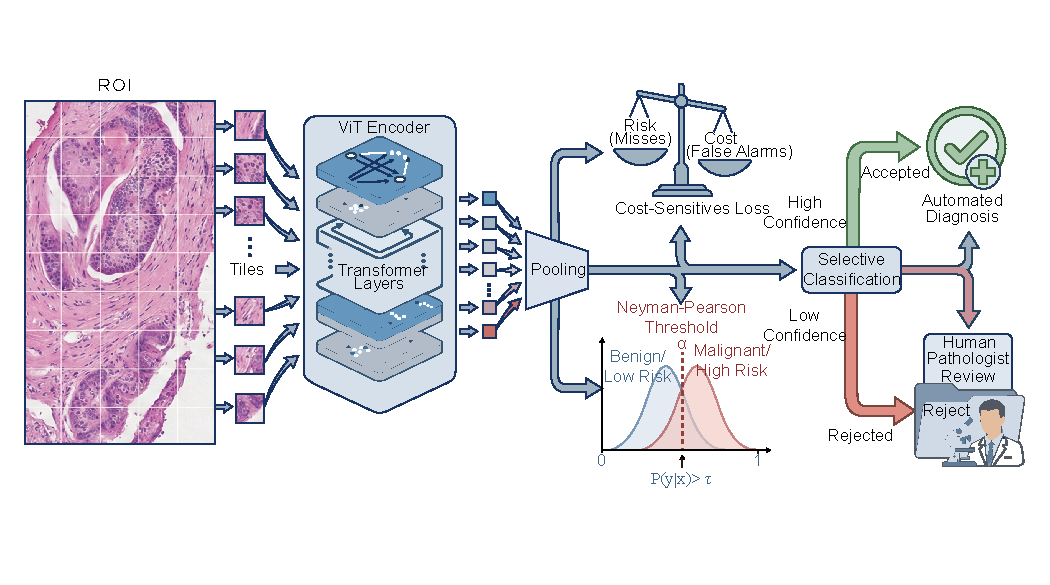
\includegraphics[scale=0.95]{figures/frame_figure.pdf}
  \caption{Overview of the three-phase framework. (a) A ViT-based MIL baseline; (b) cost‑sensitive learning with threshold calibration to control false‑negative risk; (c) selective classification that abstains on uncertain samples for human review.}
  \label{fig:framework}
\end{figure*}


We frame MIP identification as a binary multiple instance learning (MIL) problem. A pathology image is partitioned into local tiles via a sliding window and represented as a bag \( X_i = \{\mathbf{x}_{i,1}, \dots, \mathbf{x}_{i,n_i}\} \), where the bag size \( n_i \) may vary across images. Each image is assigned an image-level label \( y_i \in \{0,1\} \), with \( y_i = 1 \) indicating MIP presence and \( y_i = 0 \) its absence. The objective is to learn a bag-level classifier \( f(X) \) that predicts the probability \( \hat{p} = \mathbb{P}(y = 1 \mid X) \), while explicitly constraining the false negative rate (FNR) for the high-risk positive class.

\subsection{The Backbone: ViT-based MIL with Gated Attention Pooling}
\label{sec:baseline_method}

We use a Vision Transformer (ViT) \cite{dosovitskiy2020image} as the instance encoder, followed by an attention-based pooling operator \cite{ilse2018attention} to aggregate instance features into a bag-level prediction. The following subsections present our model architecture and training protocol.

\subsubsection{Tile extraction}

\textcolor{green}{Following standard practice in computational pathology MIL, each microscopy image is decomposed into a bag of overlapping local tiles using a sliding window \cite{campanella2019clinical,lu2021data}. We load images as RGB via OpenCV \cite{bradski2000opencv} and substitute loading failures with zero-valued placeholders. Each image is padded to a minimum size of $512\times512$ using reflection padding, and we extract tiles of size 512 with a stride of 256. To preserve peripheral tissue, the final tile is aligned with the image boundary whenever the regular stride would otherwise leave uncovered margins.}\\
\textcolor{magenta}{This part is repeated with the green-marked text on Line 312.}

\subsubsection{Feature encoding}

We adopt a ViT-Base encoder pre-trained using the Phikon framework \cite{filiot2023scaling}. \textcolor{green}{The backbone consists of 12 transformer layers with hidden dimension \( d = 768 \) and 12 attention heads (patch size 16, input resolution \(224\times224\)). We load the pre-trained weights via partial key-matching,}\textcolor{magenta}{This part is repeated with the green-marked text on Line 314.} and extract the \([CLS]\) token embedding from the final layer as the tile-level representation. Thus, for tile \(\mathbf{x}_k\), the instance feature is obtained as:
\begin{equation*}
    \mathbf{h}_k = f_{\text{ViT}}(\mathbf{x}_k; \theta_{\text{enc}}), \quad \mathbf{h}_k \in \mathbb{R}^{768}.
\end{equation*}

\subsubsection{Gated attention pooling and bag-level prediction}\label{S3-1-3}
We aggregate tile features using a gated attention mechanism \cite{ilse2018attention}. For a bag of features \( H_i = \{\mathbf{h}_{i,j}\}_{j=1}^{n_i} \) from the \( i \)-th image, unnormalized attention scores \( s_{i,j} \) are computed as:
\begin{equation*}
    s_{i,j} = \mathbf{w}^\top \Bigl(\tanh(V\mathbf{h}_{i,j}) \odot \sigma(U\mathbf{h}_{i,j})\Bigr),
\end{equation*}
where \( V, U \in \mathbb{R}^{256 \times 768} \) and \( \mathbf{w} \in \mathbb{R}^{256} \) are learnable parameters. These scores are normalized via softmax to produce attention weights \( a_{i,j} \). \textcolor{green}{In practice, bags are padded to the maximum size within a batch, and a boolean mask identifies valid tiles.}\textcolor{magenta}{This is identical to the second green-highlighted text in Line 312.}

The bag-level representation is then given by:
\begin{equation*}
    \mathbf{z}_i = \sum_{j=1}^{n_i} a_{i,j} \mathbf{h}_{i,j} \in \mathbb{R}^{d}.
\end{equation*}
Finally, a linear classifier \( h_{\mathrm{c}}: \mathbb{R}^{d} \to \mathbb{R} \) projects \( \mathbf{z}_i \) to a logit, which is passed through a sigmoid to yield the predicted probability \(\hat{p}_i = \sigma(h_{\mathrm{c}}(\mathbf{z}_i))\).

\subsection{Phase I: Risk-Aware Training via Cost-Sensitive Learning}\label{sec:phase1_method}

While the baseline model follows a standard training objective that minimizes average classification error, this approach overlooks the clinical asymmetry of risks: false negatives (FN) are considerably more costly than false positives (FP) in high‑stakes diagnostic settings. To incorporate this asymmetry directly into representation learning, we adopt a cost‑sensitive learning (CSL) strategy to enforce higher penalties on false negatives \cite{he2009learning}.  Let \(\mathcal{D} = \{(X_i, y_i)\}_{i=1}^{n}\) denote the training set, where \(y_i \in \{0,1\}\) indicates the label (1 for MIP‑present, 0 for MIP‑absent) and \(\hat{p}_i\) is the predicted positive probability. The cost‑sensitive loss is defined as  
\begin{equation*}
    \mathcal{L}_{\mathrm{cs}} = - \frac{1}{n} \sum_{i=1}^{n} \Bigl[ w_{1} \, y_i \log(\hat{p}_i) + w_{0} \, (1-y_i) \log(1-\hat{p}_i) \Bigr].
\end{equation*}
The weight \(w_{0}=1.0\) is kept for the majority negative class, while \(w_{1} > 1\) is a hyper‑parameter that scales the penalty for missing a positive case.  
In practice, we implement this by passing class weights \([w_{0}, w_{1}]\) (i.e., \([1, w_{1}]\)) to the cross‑entropy function, thereby amplifying gradients from positive samples during back‑propagation.


\subsection{Phase II: Strict Risk Control via Neyman-Pearson Paradigm}
\label{sec:phase2_method}

Cost‑sensitive learning increases sensitivity but cannot guarantee a distribution‑free bound on the false‑negative risk. To enforce strict control over false negatives at inference, we employ a Neyman–Pearson (NP) threshold‑calibration procedure \cite{rigollet2011neyman,tong2018neyman}. Rather than using a fixed threshold (\(\tau = 0.5\)), we calibrate \(\tau\) on a held‑out set of positive samples via a classical non‑parametric order‑statistics method, constructing a tolerance limit on the false‑negative rate \cite{wilks1941determination}.

We hold out a calibration set $\mathcal{D}_{\mathrm{cal}}$ of $m_1$ positive samples from training. Let $\hat{p} = f(X)$ be the predicted probability of the positive class. The scores $\{\hat{p}_i\}_{i=1}^{m_1}$ on $\mathcal{D}_{\mathrm{cal}}$ are sorted as $\hat{p}_{(1)} \le \cdots \le \hat{p}_{(m_1)}$. For a threshold $\tau$, the decision rule $\hat{y} = \mathbb{I}(\hat{p} \ge \tau)$ yields the population false negative rate
\[
\mathrm{FNR}(\tau) = \mathbb{P}(\hat{p} < \tau \mid y = 1).
\]

\begin{theorem}[Finite-sample FNR Control via NP Umbrella]\label{Th1}
For a target risk level $\alpha\in(0,1)$ and tolerance $\delta\in(0,1)$, we select an index $k$ such that the corresponding binomial tail probability is bounded by $\delta$, and set $\hat{\tau}_{\alpha,\delta} = \hat{p}_{(k)}$. Under the assumption that calibration positives are i.i.d. from the true positive distribution, the resulting classifier constructed by the NP umbrella procedure satisfies the Neyman-Pearson risk control guarantee,
\[
\mathbb{P}\bigl(\mathrm{FNR}(\hat{\tau}_{\alpha,\delta}) > \alpha\bigr)
\leq \delta,
\]
In other words, with confidence at least $1-\delta$, the false negative rate (FNR) on the test distribution does not exceed $\alpha$.
\end{theorem}

\begin{remark}
The guarantee is distribution-free, holds in finite samples, and is invariant to model complexity. Following a strict Neyman--Pearson framework, it ensures the false-negative risk is bounded for any scoring function---whether a CNN, Vision Transformer, or cost-sensitive model---without retraining or architectural change. In clinical terms, this provides $1-\delta$ confidence that the missed-diagnosis rate will not exceed $\alpha$, delivering an operational safety guarantee that is stronger and more interpretable than average-accuracy measures. The proof of Theorem \ref{Th1} is delegated to Appendix \ref{S6-1}.
\end{remark}


\subsection{Phase III: Selective Classification via Conformal Risk Control}\label{sec:phase3_method}

We propose a hybrid framework that unifies theoretical risk modeling, selective optimization, and rigorous post-hoc calibration. Built upon the learning-theoretic guarantees of selective classification, our method employs a deep neural network for approximation and is strictly calibrated to ensure clinical safety.

For a selective classifier $(f,g)$, the empirical risk is defined as
\[
\hat{R}_n(f,g) = \frac{\frac{1}{n} \sum_{i=1}^n \ell(y_i, f(X_i)) \cdot g(X_i)}
{\hat{\Phi}_n},
\]
where $\hat{\Phi}_n = \frac{1}{n} \sum_{i=1}^n g(X_i)$ is the empirical coverage.
The corresponding population risk is given by
\[
R(f,g) = \mathbb{E}\bigl[\ell(y, f(X)) \mid g(X) = 1\bigr],
\]
which represents the expected loss conditioned on the classifier accepting the sample.
\begin{theorem}[Coverage Guarantee with Risk Tolerance]\label{Th2}
Assume that $\mathcal{F}$ is finite, and let $(f,g)$ be a selective classifier selected by the generalized consistent selective strategy (CSS) procedure, satisfying the empirical risk condition $\hat{R}_n(f,g) \leq \epsilon/2$. Then, for any $0 \leq \delta \leq 1$, with probability at least $1-\delta$, the following two conditions hold simultaneously:
\begin{enumerate}
    \item Risk Upper Bound: 
    \[R(f,g) \leq \epsilon.
    \]
    \item Coverage Lower Bound:
    \[
    \Phi(f,g) \geq 1 - \frac{2}{n} \left( \ln 2 \cdot 1.58\min\{|\mathcal{F}|, |\mathcal{X}|\} + \ln \frac{2}{\delta} \right) - \epsilon.
    \]
\end{enumerate}
\end{theorem}
\begin{remark}[Remark for Theorem \ref{Th2}.]
Theorem \ref{Th2} extends the zero-risk result of \cite{el2010foundations} to a more practical $\epsilon$-risk setting, establishing a formal risk–coverage tradeoff for selective classification. This guarantee enables practitioners to safely adjust the reject threshold while maintaining a theoretically bounded error rate. The proof of Theorem \ref{Th2} is presented in Appendix \ref{S6-2}.
\end{remark}

Motivated by the risk-coverage trade-off formalized in Theorem \ref{Th2}, we implement the selective classification mechanism $(f,g)$ via a deep neural network. To this end, we design three output heads:

\begin{itemize}
\item \textbf{Prediction head $f(\cdot)$}: A classification head that outputs class probabilities $\mathbf{p} \in \mathbb{R}^{K-1}$, where $K$ denotes the number of classes. This head is used to generate the final predictive label $\hat{y}$.
\item \textbf{Selection head $g(\cdot)$}: A parallel head that produces a scalar confidence score $g(\cdot) \in [0,1]$, which estimates the reliability of the prediction. This score is thresholded to implement a selective abstention mechanism: if $g(\cdot) \ge \tau$, the prediction is accepted; otherwise, the model abstains from making a decision.
\item \textbf{Auxiliary head} $h(\cdot)$: Trained on the standard classification objective to stabilize representation learning and regularize the overall model.
\end{itemize}

We formulate a differentiable objective to approximate the constraints in Theorem \ref{Th2}. The empirical selective risk $\hat{R}_n(f,g)$ is computed using cross-entropy loss $\ell$ \cite{geifman2019selectivenet}. To enforce a target coverage $c$, we introduce a quadratic penalty $\Psi(g) = \beta \max\big(0, c - \hat{\Phi}_n \big)^2$, where $\beta$ controls the constraint weight. Starting from the bag-level representation $\mathbf{z} \in \mathbb{R}^d$ introduced in Subsection \ref{S3-1-3}, the overall loss is defined as:
\begin{equation*}
    \mathcal{L} = \gamma \left(\hat{R}_n(f,g) + \Psi(g)\right) + (1-\gamma) \ell_{\mathrm{ce}}(h(\mathbf{z}_i), y_i),
\end{equation*}
where $\gamma$ balances between selective optimization and auxiliary classification, mirroring the role of the theoretical risk bound $\epsilon$. Minimizing $\mathcal{L}$ encourages the model to select samples with low prediction error, driving $\hat{R}_n(f,g)$ toward the theoretical guarantee. We then introduce four cases to achieve explicit control over risk and/or false negative rate (FNR).

\textbf{Case 1: Risk Control.}
Empirical threshold selection via calibration:
\[
\hat{R}(\tau)=\frac{\sum_{i\in\mathcal{S}_\tau}\mathbb{I}(\hat{y}_i \neq y_i)}{|\mathcal{S}_\tau|},
\quad
\mathcal{S}_\tau=\{i\in\mathcal{D}_{\mathrm{cal}}\mid g(X_i)\geq \tau\}.
\]
The optimal threshold $\tau_{1}^*$ is selected on the calibration set as
\begin{equation}\label{Eq1}
    \tau_{1}^*=\inf\{\tau \in[0,1]\mid\hat{R}(\tau)\leq\alpha\}.
\end{equation}
This yields the selective classifier
\[
(f,g)_{\tau_{1}^*}(X)=
\begin{cases}
\mathbb{I}\!\left(f(X)>0.5\right), & g(X)\geq \tau_{1}^*,\\[4pt]
\text{abstain}, & \text{otherwise}.
\end{cases}
\]

\textbf{Case 2: False Negative Rate Control.}
The empirical false negative rate (FNR) is estimated on a calibration set as
\[
\widehat{\mathrm{FNR}}(\tau)=\frac{\sum_{i \in\mathcal{S}_\tau}\mathbb{I}(\hat{y}_i=0\,\wedge\, y_i=1)}{|\{i\in\mathcal{D}_{\mathrm{cal}}\mid y_i=1\}|},
\]
where only positive-labeled samples are considered in the denominator. To control FNR below level $\alpha$, we select the optimal threshold via 
\begin{equation}\label{Eq2}
  \tau_{2}^*=\inf\{\tau\in[0,1]\mid \widehat{\mathrm{FNR}}(\tau)\leq\alpha\}.  
\end{equation}

\begin{remark}
The fundamental distinction between $\tau_{1}^{*}$ in Eq. \ref{Eq1} and $\tau_{2}^{*}$ in Eq. \ref{Eq2} lies in the criterion used for threshold selection: overall risk versus false negative rate (FNR). By choosing the appropriate selection rule according to the clinical context, we can align the model's abstention behavior with domain-specific reliability requirements, thereby enabling truly trustworthy diagnostic support.
\end{remark}

The resulting selective classifier abstains when the confidence score falls below $\tau_{2}^*$:
\[
(f,g)_{\tau_{2}^*}(X)=
\begin{cases}
\mathbb{I}\!\left(f(X)>0.5\right), & g(X)\geq \tau_{2}^*,\\[4pt]
\text{abstain}, & \text{otherwise}.
\end{cases}
\]


\textbf{Case 3: Risk Control with Cost-sensitive Learning.}

Selective inference typically pursues two objectives: controlling a risk measure while maximizing coverage. In the context of lung adenocarcinoma subtype classification, we introduce a third clinical requirement: controlling the FNR. While the threshold \(\tau_{1}^{*}\) derived from Case 1 ensures risk control, it may fail to satisfy clinical FNR constraints. To address this, we integrate the cost-sensitive learning strategy outlined in Section \ref{sec:phase1_method}, training a classifier that is explicitly sensitive to false negatives during the training phase. This approach enables a clinically meaningful trade‑off among the three objectives: risk control, FNR control, and coverage maximization.

\textbf{Case 4: False Negative Control with Cost-sensitive Learning.}

While Case 2 effectively controls the FNR, it may do so at the cost of unacceptably low coverage. This occurs because the model treats false negatives and false positives equally during training, failing to recognize the clinical severity of missing a positive case. Consequently, the resulting threshold tends to be overly aggressive, leading to high abstention rates and placing a substantial review burden on human experts. A natural remedy, analogous to the approach in Case 3, is to incorporate cost‑sensitive learning during training. By penalizing false negatives more heavily, the model learns to reduce such errors, which in turn yields a more conservative threshold and thereby improves coverage while maintaining strong FNR control.

\section{Experiments and Results}\label{sec:experiments}

\textcolor{red}{
All questions：
1. Lines 296–300 in Section 4.1 contain substantial duplicated content.
The two passages are nearly verbatim repetitions of the following settings:
- AdamW optimizer (learning rate of $1\times10^{-5}$, weight decay of 0.05)
- Training scheme: 15 epochs with cosine annealing and linear warm-up
- Mixed-precision training combined with gradient accumulation
- Dropout rate of 0.2 and label smoothing of 0.1
- Normalization using ImageNet statistics
- Data augmentation configurations (224×224 input size, flipping, rotation, and color jitter)\\
2. Section 4.1 lacks information on dataset class distribution.
The numbers of positive and negative samples are not specified (1519 positive versus 5614 negative, with an approximate ratio of 1:3.7).\\
3. Section 4.1 lacks a general overview of the validation strategies.
Different experimental settings adopt distinct validation protocols: the Baseline and CSL models use standard 5-fold cross-validation; NP and CSL+NP adopt ten repeated Monte Carlo Cross-Validation (MCCV); SelectiveNet employs 5-fold cross-validation combined with swap calibration. We suggest providing a unified description of all validation strategies in Section 4.1, rather than introducing them separately at the beginning of each subsection. In addition, swap calibration is applied to all experimental cases of SelectiveNet.\\
4. The validation description at Line 306 in Section 4.2 is redundant with Section 4.1.
The sentence *“We performed a stratified 5-fold cross-validation at the image level”* in Line 306 has already been stated in Line 298 of Section 4.1.\\
5. Section 4.3 contains overly lengthy descriptions of competing models. Detailed algorithm illustrations for CLAM-SB, DS-MIL, DTFD-MIL, and TransMIL each occupy 4–6 lines. Since these are well-established published methods, their introductions can be appropriately condensed into brief summaries.\\
6. Section 4.3, Line 439: "Phase II introduces Neyman–Pearson..."
The subsection title already corresponds to Phase II, and the MCCV procedure has been elaborated in Lines 430–437. The statement "Phase II introduces..." constitutes a redundant third introduction of the same content.}

In this section, we systematically evaluate the proposed framework through a cascade of eight complementary experiments. We first describe the experimental setup in Subsection \ref{S3-1} and then report the performance of our baseline model in Subsection \ref{S3-2}, followed by comparisons with competing state-of-the-art MIL architectures in Subsection \ref{S3-3}. To address the inherent limitations of architectural design alone, we progressively investigate three phases: risk-aware training via cost-sensitive learning in Subsection \ref{sec:phase1_results}, threshold selection via NP calibration in Subsection \ref{sec:phase2_results}, and the synergistic effect of cost-sensitive learning boosting NP calibration in Subsection \ref{S3-4}. We further extend to selective classification with conformal risk or FNR control in Subsection \ref{sec:phase3_results}, and conclude with external validation in Subsection \ref{S3-6}. Together, these subsections form a coherent progression from standard benchmarking to risk-controllable and reliable decision-making.
\textcolor{blue}{I will mark the repeated content within Chapter Four in cyan. Please do not confuse it with green highlights, which indicate duplicated content between Chapter Three and Chapter Four.}
\subsection{Experimental Setup}\label{S3-1}

We implement our framework in PyTorch and run all experiments on an NVIDIA RTX 5090 GPU (32 GB). The dataset consists of 7,133 locally collected pathology images with image-level labels indicating MIP-present ($y = 1$) or MIP-absent ($y = 0$). Following common practice in computational pathology \cite{campanella2019clinical,lu2021data}, \textcolor{green}{we partition each image into overlapping $512 \times 512$ tiles using a sliding window of stride 256. Reflection padding is applied at boundaries to ensure full coverage.} Each tile is resized to $224 \times 224$ to preserve tissue-level context. \textcolor{green}{To handle variable bag sizes in mini-batches, we use zero-padding with an attention mask that excludes padded regions from gradient updates.} Input tiles are normalized using ImageNet statistics. During training, we apply strong data augmentation via Albumentations \cite{buslaev2020albumentations}, including random flips, moderate rotations, and color jitter.

\textcolor{green}{We initialize the ViT-based MIL baseline with Phikon weights \cite{filiot2023scaling} and employ gated attention pooling \cite{ilse2018attention}.} \textcolor{cyan}{Optimization uses AdamW \cite{loshchilov2017decoupled} with learning rate $1 \times 10^{-5}$ and weight decay $0.05$ for 15 epochs, following a cosine schedule with linear warmup. Training employs mixed precision \cite{micikevicius2017mixed} and gradient accumulation (effective batch size 32 over 4 steps). We use cross-entropy loss with label smoothing $0.1$ \cite{szegedy2016rethinking} and dropout $0.2$ in the classification head.}\textcolor{magenta}{This part is repeated with the cyan-marked text on Line 324.}

\textcolor{cyan}{We adopt an image-level stratified 5-fold cross-validation.}\textcolor{magenta}{This part is repeated with the cyan-marked text on Line 324.} In addition to standard metrics (AUC and accuracy), we report ROC/PR curves and conduct calibration analysis using reliability diagrams and Brier scores \cite{guo2017calibration}. Unless stated otherwise, results are reported using the final training checkpoint with a default decision threshold $\tau = 0.5$.

\textcolor{cyan}{To ensure stable and reproducible evaluation, we fix random seeds and enable deterministic cuDNN. The dataset is split into 80\% training and 20\% test using stratified sampling. All models are optimized with the same protocol: AdamW \cite{loshchilov2017decoupled} ($10^{-5}$, weight decay $0.05$) for 15 epochs, cosine schedule with 10\% linear warmup \cite{loshchilov2016sgdr}, mixed precision, and gradient accumulation (batch size 8, accumulation steps 4). Dropout $0.2$ and label smoothing $0.1$ are applied for regularization \cite{szegedy2016rethinking}. Each tile is normalized with ImageNet statistics \cite{russakovsky2015imagenet} and augmented via resizing to $224 \times 224$, random flips, rotation $\pm 15^\circ$, and color jitter. }

\subsection{Baseline Model Performance}\label{S3-2}

In clinical practice, pathologists often inspect specific high-magnification regions of interest (ROIs) to identify subtle histological growth patterns. These ROIs, however, typically exceed the input size constraints of standard neural networks. Consequently, we adopt the multiple instance learning (MIL) paradigm, which aggregates tile-level features into a whole-slide prediction without requiring pixel-level annotations.

\textcolor{cyan}{We performed a stratified 5-fold cross-validation at the image level.} In each fold, the ViT‑MIL model was re‑initialized from the same Phikon checkpoint and trained for 15 epochs under identical optimization settings. Evaluation was conducted on the held‑out fold using the last‑epoch model with a fixed threshold $\tau = 0.5$. 

\begin{figure}[htbp]
    \centering
    \subfloat[Confusion matrix]{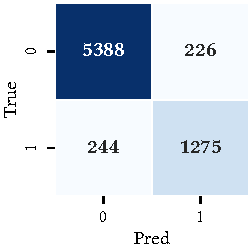
\includegraphics[scale=0.9]{figures/Tiny_CM.pdf}}
    \hspace{0.1cm}
    \subfloat[ROC curve]{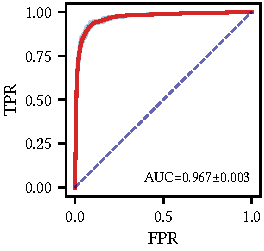
\includegraphics[scale=0.9]{figures/Tiny_ROC.pdf}}
    \caption{Confusion matrix and ROC curve of baseline model.}
    \label{fig:cv_plots}
\end{figure}

For each cross‑validation run, we compute the area under the ROC curve (AUC) from predicted probabilities and classification accuracy from thresholded predictions. Table~\ref{tab:cv_results} reports the mean $\pm$ standard deviation across all five folds. Figure~\ref{fig:cv_plots} displays the mean ROC curve, obtained by interpolating fold‑wise true positive rates (TPR) onto a common false positive rate (FPR) grid; the shaded region indicates $\pm 1$ standard deviation across folds. Additionally, we provide an aggregated confusion matrix by concatenating predictions from all folds.

\begin{table}[htbp]
    \centering
    \caption{The prediction performance of baseline model.}
    \label{tab:cv_results}
    \resizebox{85mm}{!}{
    \begin{tabular}{ccccc}
    \toprule
    Fold & ACC & AUC & FNR & FPR \\
    \midrule
    1 & 93.06\% & 96.93\% & 18.09\% & 3.92\% \\
    2 & 93.06\% & 96.41\% & 18.42\% & 3.83\% \\
    3 & 92.92\% & 96.94\% & 14.47\% & 5.08\% \\
    4 & 94.04\% & 96.81\% & 16.78\% & 3.03\% \\
    5 & 93.97\% & 97.23\% & 12.54\% & 4.27\% \\
    \midrule
    Mean & 93.41\% & 96.87\% & 16.06\% & 4.03\% \\
    Std & $\pm$ 0.60\% & $\pm$ 0.30\% & $\pm$ 2.51\% & $\pm$ 0.74\% \\
    \bottomrule
    \end{tabular}
    }
\end{table}

As shown in Figure \ref{fig:cv_plots}, while the AUC remains consistently high and stable (mean $0.97 \pm 0.003$), the baseline reveals a systematic failure on the high‑stakes positive class: across the five folds, a total of 244 false negatives were observed. Table~\ref{tab:cv_results} further quantifies this instability, with the false negative rate (FNR) exhibiting notable fluctuation (mean $16.06\%$, std $\pm 2.51\%$). These results highlight the model's weak reliability in detecting clinically critical cases, despite strong aggregate discriminative performance.


\subsection{Comparison with Competing Models}\label{S3-3}

Existing state-of-the-art MIL architectures (e.g., CLAM-SB, DS-MIL, DTFD-MIL, TransMIL) are originally designed for whole-slide image (WSI) classification, which involves large bag sizes and macro-level sparsity. In contrast, our clinical task focuses on region-of-interest (ROI) microscopy images, which exhibit denser morphological patterns and highly localized spatial contexts. To establish a fair benchmark, we adapt these aggregators into a unified ROI-optimized pipeline: all models take identical Phikon-encoded \cite{filiot2023scaling} tile features $H_i = \{h_{i,j}\}_{j=1}^{n_i} \in \mathbb{R}^{n_i \times d}$ ($d=768$) as input, preserving their core aggregation algorithms while standardizing tile extraction and feature encoding, thereby decoupling feature representation from aggregation mechanism. The competing models are summarized as follows:


\begin{itemize}
    \item \textbf{CLAM-SB} (Clustering-constrained-attention MIL) \cite{lu2021data}: It augments standard attention with an instance-level clustering objective. Its attention network employs a gated mechanism to obtain bag-level representations. Additionally, CLAM-SB selects the most highly attended patches (Top-$k$) to generate pseudo-labels, jointly optimizing a bag-level classification loss and an instance-level clustering loss. This auxiliary supervision linearly separates critical micropapillary (MIP) patterns from benign background tissues in the feature space.
    
    \item \textbf{DS-MIL} (Dual-stream Multiple Instance Learning) \cite{li2021dual}: It employs a dual-stream architecture to jointly capture extreme local anomalies and global morphological context. The first stream selects the most discriminative instance feature via max-pooling, identified by the highest positive predictive score. The second stream applies a non-local attention mechanism that computes pairwise similarities between this critical instance and all other tiles in the bag. The two streams produce complementary representations, which are concatenated and passed to a classifier for the final diagnostic prediction, offering a calibrated global-local perspective.
    
    \item \textbf{DTFD-MIL} (Double-Tier Feature Distillation) \cite{zhang2022double}: It addresses the challenge of extreme bag size variance through a double-tier distillation paradigm. It first randomly partitions each variable-length bag into a fixed number of pseudo-bags. In the first tier, a local attention mechanism aggregates patches within each pseudo-bag to produce intermediate representations, which are directly supervised by the bag label. In the second tier, a global attention network aggregates these pseudo-bag features into the final slide-level representation. This hierarchical distillation effectively amplifies the perceptible signal from minority MIP regions.
    
    \item \textbf{TransMIL} (Transformer based Correlated MIL) \cite{lu2021data, shao2021transmil}: It departs from the independent and identically distributed (i.i.d.) assumption of conventional MIL by formulating bag classification as sequence modeling. It compresses the bag representation into a 512-dimensional sequence and prepends a learnable \texttt{[CLS]} token. To capture spatial correlations, TransMIL introduces a Pyramid Position Encoding Generator (PPEG), which reshapes the 1D sequence into a 2D grid and applies multi-scale depth-wise convolutions (e.g., $3 \times 3$, $5 \times 5$, $7 \times 7$) to model macroscopic architectural context. The resulting sequence is then processed by standard Transformer encoder layers, with the final prediction derived directly from the aggregated \texttt{[CLS]} token.
\end{itemize}


\begin{table}[htbp]
    \centering
    \caption{Performance comparison of baseline and other competing models.}\label{tab:sota_comparison}
    \resizebox{85mm}{!}{
    \begin{tabular}{lcccc}
        \toprule
        Model & ACC & AUC & FNR & FPR \\
        \midrule
        Baseline & \textbf{93.41\%} & \textbf{96.87\%} & 16.06\% & \textbf{4.03\%} \\
                 & $\pm$ 0.60\% & $\pm$ 0.30\% & $\pm$ 2.51\% & $\pm$ 0.74\% \\
        \midrule
        CLAM-SB  & 93.34\% & 96.36\% & 16.32\% & 4.04\% \\
                 & $\pm$ 0.90\% & $\pm$ 0.71\% & $\pm$ 2.77\% & $\pm$ 0.62\% \\
        \midrule
        DS-MIL   & 92.92\% & 96.28\% & 16.92\% & 4.42\% \\
                 & $\pm$ 0.80\% & $\pm$ 0.70\% & $\pm$ 3.19\% & $\pm$ 0.82\% \\
        \midrule
        DTFD-MIL & 93.23\% & 96.49\% & 16.72\% & 4.08\% \\
                 & $\pm$ 0.76\% & $\pm$ 0.47\% & $\pm$ 2.08\% & $\pm$ 0.62\% \\
        \midrule
        TransMIL & 93.16\% & 96.15\% & \textbf{15.67\%} & 4.45\% \\
                 & $\pm$ 0.64\% & $\pm$ 0.48\% & $\pm$ 2.09\% & $\pm$ 0.73\% \\
        \bottomrule
    \end{tabular}
    }
\end{table}

As shown in the table \ref{tab:sota_comparison}, the predictive performance of these competing backbones is highly similar, with accuracy around 93\% and FNR around 16\%. This suggests that architectural design alone is insufficient to achieve risk-controllable and reliable decision-making for lung adenocarcinoma classification. Therefore, while keeping the backbone architecture fixed, we next dissect this problem progressively through three phases.



\subsection{Phase I: Risk-Aware Training via Cost-Sensitive Learning}\label{sec:phase1_results}

To mitigate the high false negative rate (FNR) observed in the baseline, we adopt Cost-Sensitive Learning (CSL) \cite{he2009learning,zadrozny2004learning}. For each positive-class weight $w_{1} \in \{5,10,15,20\}$, we train the same ViT-MIL architecture using a class-weighted cross-entropy loss, with the negative-class weight fixed at $w_{0}=1$. \textcolor{cyan}{All training settings—including optimizer (AdamW, $1\times10^{-5}$ learning rate, $0.05$ weight decay), scheduler (cosine annealing with 10\% warmup), mixed precision, gradient accumulation, and 15 epochs without early stopping—are kept same to the baseline.}\textcolor{magenta}{This experimental setup appears here for the third time.In line 314 and 324.} For evaluation, we maintain the same decision threshold $\tau = 0.5$. Figure~\ref{fig:main_diagram} illustrates the overall behavior across different cost scenarios.

\begin{itemize}
    \item Confusion matrix (top row): Increasing $w_1$ makes the classifier progressively more sensitive to the positive class, generally lowering false negatives at the cost of higher false positives.
    \item Probability density (bottom row): Larger $w_1$ shifts the predicted probability distribution of positive samples (coloring in red) toward higher values, directly explaining the improved sensitivity under the fixed threshold $\tau=0.5$.
\end{itemize}

\begin{figure*}[htbp]
    \centering
    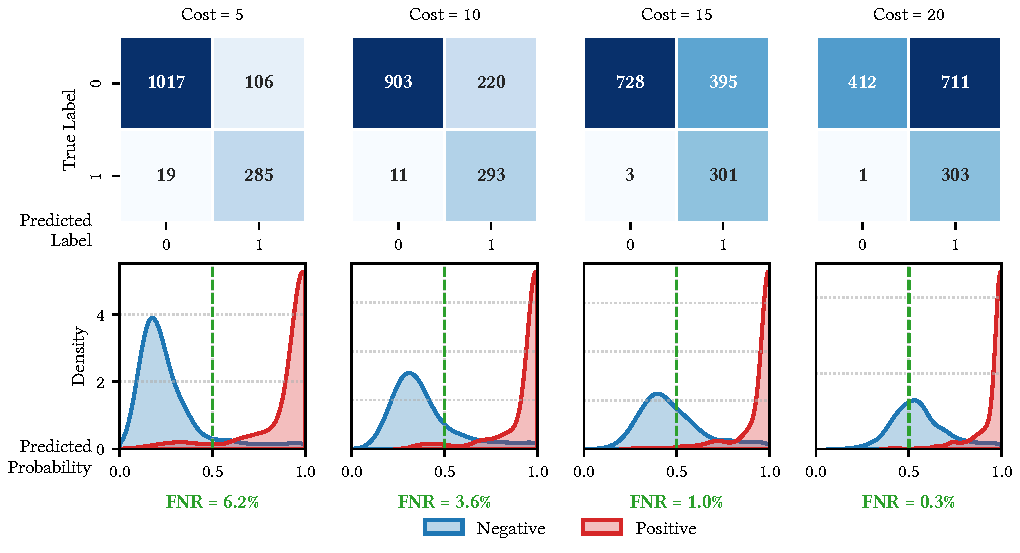
\includegraphics[width=0.85\textwidth]{figures/Final_KDD_Figure.pdf} 
    \caption{Confusion matrices and class probability densities under varying cost sensitivity.}
    \label{fig:main_diagram}
\end{figure*}

\begin{table}[htbp]
    \centering
    \caption{The prediction performance of cost-sensitive learning.}\label{tab:cost_results}
    \resizebox{70mm}{!}{
    \begin{tabular}{ccccl}          
        \toprule
        Cost & ACC & AUC & FNR & FPR \\
        \midrule
        5  & 91.24\% & 97.17\% & 6.25\% & 9.44\% \\
        10 & 83.81\% & 97.35\% & 3.62\% & 19.59\% \\
        15 & 72.11\% & 97.51\% & 0.99\% & 35.17\% \\
        20 & 50.11\% & 97.80\% & 0.33\% & 63.31\% \\
        \bottomrule
    \end{tabular}
    }
\end{table}

As shown in Table \ref{tab:cost_results}, adjusting the positive-class cost weight provides empirical control over the false negative rate (FNR), albeit at the cost of reduced overall accuracy. For example, setting the cost weight to 5 reduces the baseline FNR from 16.06\% to 6.25\% while only decreasing accuracy by 2.17\%, a trade-off that significantly mitigates clinical missed-detection risk. Although further increasing the cost penalty continues to lower the FNR, the attainable limit of such reduction remains without rigorous theoretical guarantees.


\subsection{Phase II: Threshold Selection via NP Calibration}
\label{sec:phase2_results}

To reduce variability due to calibration-set sampling, we employ a Monte Carlo cross-validation (MCCV) scheme with 10 repetitions. A fixed test set (20\% of the data) is held out, with the remaining 80\% serving as a training pool. In each repetition, we randomly sample 100 positive instances from this pool to form the calibration set \(\mathcal{D}_{\mathrm{cal}}\); the rest of the positives and all negatives are used for training. The calibration threshold is derived from \(\mathcal{D}_{\mathrm{cal}}\), and model performance is evaluated on the held-out test set.

To empirically approximate the target risk levels \(\alpha \in \{0.01, 0.05, 0.10\}\) on a calibration set of size \(m_{1}=100\), we select order‑statistic indices based on zero‑based numbering. Specifically, we choose indices \(\{0, 4, 9\}\), corresponding to the \(k\)-th smallest scores for \(k \in \{1, 5, 10\}\). The calibrated thresholds are then given by  
\[
\hat{\tau}_{0.01}=\hat{p}_{(1)},\quad 
\hat{\tau}_{0.05}=\hat{p}_{(5)},\quad 
\hat{\tau}_{0.10}=\hat{p}_{(10)}.
\]
\textcolor{magenta}{The introduction to NP here is somewhat redundant. Relevant explanations have already been elaborated in the methodology and this section, so such detailed descriptions are unnecessary.}
Phase II introduces Neyman–Pearson (NP) thresholding to obtain formal, statistically grounded risk control \cite{rigollet2011neyman,tong2018neyman}. Empirically calibrated thresholds $\hat{\tau}$ are derived for three target risk levels: $10\%$, $5\%$, and $1\%$. The resulting score distributions and prediction performance are summarized in Figure~\ref{fig:np_summary} and Table~\ref{tab:table3}.

\begin{figure}[htbp]
    \centering
    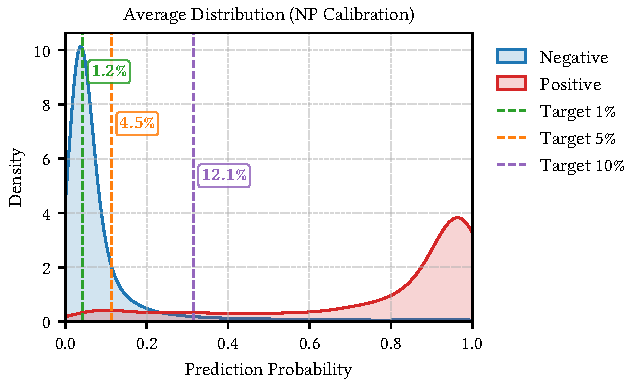
\includegraphics[width=0.95\linewidth]{figures/Final_Aggregated_Plot_NP.pdf}
    \caption{Corresponding thresholds under different FNR targets.}
    \label{fig:np_summary}
\end{figure}

\begin{enumerate}
    \item \textbf{Target 10\%:} A more relaxed threshold of $0.31$ results in an accuracy of 92.31\% but an FNR of 12.11\%.
    \item \textbf{Target 5\%:} A threshold of $0.11$ yields a balanced FNR of 4.47\% and accuracy of 82.72\%.
    \item \textbf{Target 1\%:} With a threshold of $0.04$, the FNR drops to 1.22\% (nearly all positives captured), while accuracy falls to 53.02\%.
\end{enumerate}

\begin{table}[htbp]
    \centering
    \caption{The prediction performance via NP threshold calibration.}
    \label{tab:table3}  
    \resizebox{75mm}{!}{
    \begin{tabular}{ccccl}            
        \toprule
        Strategy & ACC & AUC & FNR & FPR \\
        \midrule
        Baseline & 93.40\% & 96.53\% & 16.06\% & 4.04\% \\
        \midrule
        NP (10\%) & 92.31\% & 96.53\% & 12.11\% & 6.50\% \\
        NP (5\%)  & 82.72\% & 96.53\% & 4.47\% & 20.75\% \\
        NP (1\%)  & 53.02\% & 96.53\% & 1.22\% & 59.37\% \\
        \bottomrule
    \end{tabular}
    }
\end{table}

These results illustrate how Neyman–Pearson thresholding enables precise, statistically grounded control of the safety–efficiency trade‑off. Tighter miss‑risk targets shift the decision threshold downward, thereby lowering the false negative rate (FNR) at the expense of overall accuracy. Compared with cost-sensitive learning, NP can exactly control the false negative rate (FNR) at a specified level. However, it requires holding out a positive calibration set for threshold tuning, which not only reduces the number of samples in the training set but also exacerbates the class imbalance between positive and negative samples. This fully validates the no-free-lunch theorem.

\subsection{Enhanced Phase II: Cost-Sensitive Learning Boosting Neyman–Pearson Calibration}\label{S3-4}

Phase II confirms that Neyman–Pearson (NP) calibration can theoretically enforce a strict upper bound on the false‑negative rate (FNR). However, applying an aggressive safety target (e.g., FNR $\leq 1\%$) to the baseline model imposes a substantial practical cost: the decision threshold must be lowered drastically, leading to a false‑positive rate (FPR) of 59.37\% and a marked drop in overall accuracy.

In this phase, we examine whether cost‑sensitive learning (CSL) can serve as a more effective training precursor to Neyman–Pearson (NP) calibration. We hypothesize that because CSL explicitly penalizes false negatives during training, it shifts the predicted probability distribution of positive samples toward higher values—as observed in Phase I. Consequently, under NP calibration, a safe threshold satisfying the same target FNR should be attainable with less severe degradation in specificity compared to the baseline.

Taking the best‑performing cost‑weighted models from Phase I (\(w_{1}=5\) and \(w_{1}=10\)) as base estimators, we apply the same Monte‑Carlo cross‑validation NP calibration procedure described in Phase II. We then evaluate the calibrated thresholds under the same three risk targets: \(10\%\), \(5\%\), and \(1\%\).


\begin{table}[htbp]
    \centering
    \caption{The prediction performance with cost-sensitive learning boosting NP threshold calibration.}
    \label{tab:csl_np_results}
    \resizebox{80mm}{!}{
    \begin{tabular}{ccccl}
        \toprule
        Strategy & ACC & AUC & FNR & FPR \\
        \midrule
        \multicolumn{5}{c}{Cost-Sensitive ($w_1=5$)} \\
        \midrule
         NP (10\%) & 92.18\% & 96.50\% & 11.12\% & 6.93\% \\
         NP (5\%)  & 83.19\% & 96.50\% & 5.16\%  & 19.96\% \\
         NP (1\%)  & 53.69\% & 96.50\% & 1.91\%  & 58.33\% \\
        \midrule
        \multicolumn{5}{c}{Cost-Sensitive ($w_1=10$)} \\
        \midrule
         NP (10\%) & 92.26\% & 96.76\% & 10.46\% & 7.01\% \\
         NP (5\%)  & 85.91\% & 96.76\% & 5.33\%  & 16.46\% \\
         NP (1\%)  & 51.28\% & 96.76\% & 1.02\%  & 61.63\% \\
        \bottomrule
    \end{tabular}
    }
\end{table}

The probability density plots and threshold annotations under different cost weights are provided in Figures \ref{fig:np_cost_5_summary} and \ref{fig:np_cost_10_summary}. As shown in Table \ref{tab:csl_np_results}, compared to naive threshold adjustment in Table \ref{tab:table3}, cost‑sensitive learning substantially improves model accuracy. For instance, under the target FNR of 5\%, both $w_{1}=5$ and $w_{1}=10$ successfully control FNR at the desired level, while also raising accuracy by 0.47\% and 3.19 \%, respectively. These improvements meaningfully mitigate clinically relevant misdiagnosis rates.

\begin{figure}[htbp]
    \centering
    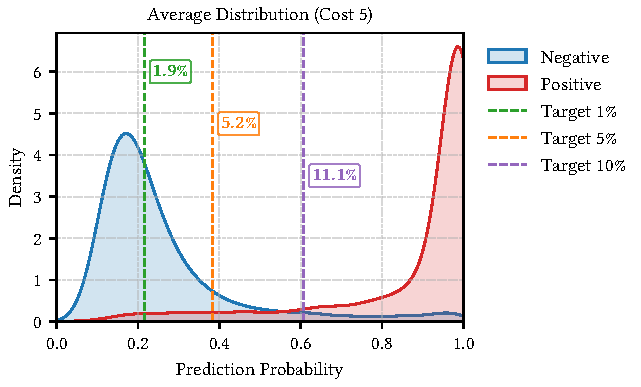
\includegraphics[width=0.95\linewidth]{figures/Final_Aggregated_Plot_Cost_5.pdf}
    \caption{Probability distribution of positive and negative samples under cost-sensitive learning ($w_1=5$). The density of predicted probabilities for positive samples (red) and negative samples (blue), along with the order-statistic thresholds (dashed lines) determined by NP calibration. Compared to the baseline, the positive distribution is shifted towards higher scores, allowing for safer thresholds with better specificity.}
    \label{fig:np_cost_5_summary} 
\end{figure}

\begin{figure}[htbp]
    \centering
    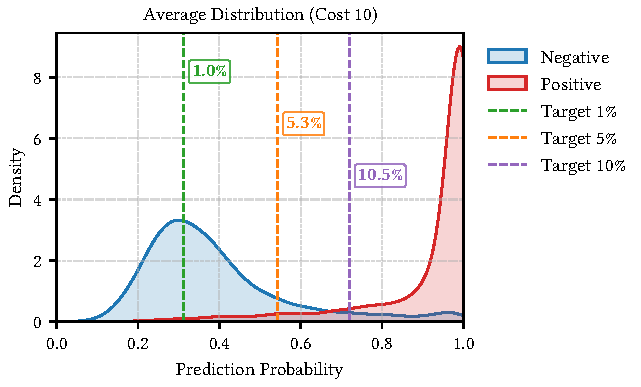
\includegraphics[width=0.95\linewidth]{figures/Final_Aggregated_Plot_Cost_10.pdf}
    \caption{Probability distribution of positive and negative samples under cost-sensitive learning ($w_1=10$). Compared to the setting with $w_1 = 5$, the distribution of positive examples shifts further to the right under $w_1 = 10$, indicating that the model becomes more inclined to predict positive for unseen samples. With the higher cost weight, the false negative rate (FNR) can be controlled more tightly: the lowest achievable test‑set FNR is $1.9\%$ for $w_1 = 5$, whereas it reduces to $1.0\%$ for $w_1 = 10$, thereby substantially lowering the risk of missed diagnoses.}
    \label{fig:np_cost_10_summary} 
\end{figure}



\subsection{Phase III: Selective Classification via Conformal Risk and/or FNR Control } \label{sec:phase3_results}

A Multiple-Instance Learning (MIL) model with an explicit reject option, following the SelectiveNet architecture, is implemented. The model is trained to minimize the empirical selective risk $\hat{R}_n(f,g)$ under a coverage constraint. The empirical coverage $\hat{\Phi}_n$ is estimated as the average selection score within each mini-batch. To satisfy $\hat{\Phi}_n \ge c$, we set the target coverage $c = 0.80$ and apply a quadratic penalty term weighted by $\beta = 32$. This penalty actively discourages acceptance rates below the 80\% threshold during training. The total training loss $\mathcal{L}$ balances selective risk minimization with an auxiliary regularization head $h(\cdot)$, using a factor $\gamma = 0.5$ to weight both terms equally.
 
To ensure statistical reliability of the empirical threshold $\tau^*$, we employ a Stratified 5-Fold Cross-Validation scheme with a Swap-Calibration strategy. In each fold, the held-out validation set is split into two disjoint subsets $\mathcal{D}_A$ and $\mathcal{D}_B$. Two independent evaluations are performed per fold: first, calibrating $\tau^*$ on $\mathcal{D}_A$ and evaluating on $\mathcal{D}_B$; second, swapping the roles by calibrating on $\mathcal{D}_B$ and evaluating on $\mathcal{D}_A$. This yields $10$ independent assessments in total, ensuring that reported safety metrics—Risk and Coverage—are computed strictly on held-out data, thereby reducing variance due to calibration.

Following the above implementation and evaluation setup, experiments are organized into two clinical paradigms shown in Figure \ref{F1}. Cases 1 and 3 target general reliability by calibrating the model to satisfy a Risk Target $\alpha \in \{1\%, 3\%, 5\%, 10\%\}$. In contrast, Cases 2 and 4 emphasize sensitivity, enforcing a False Negative Rate (FNR) Target with the same $\alpha$ values to reduce missed diagnoses. The workflows and comparative results of the four cases are summarized in Figure \ref{F1}.

\begin{figure*}[htbp]
  \centering
  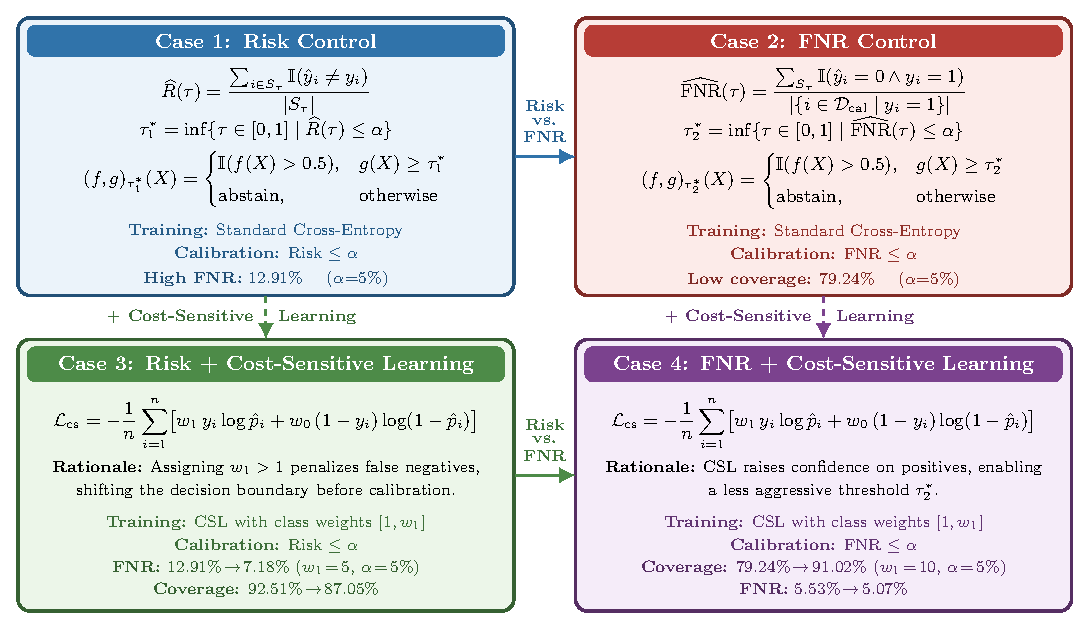
\includegraphics[scale=0.95]{figures/SC.pdf}
  \caption{The comparison of selective classification with Risk \& FNR control.}
  \label{F1}
\end{figure*}

\subsubsection{\textbf{Case 1: Selective Classification with Risk Control}}
\label{sec:case1_results}

Table~\ref{tab:table5} demonstrates the trade-off between reliability (risk) and system efficiency (coverage). Under strict risk control ($\alpha=1\%$), the model achieves a test risk of $1.48\%$, closely aligning with the $1\%$ bound, at the expense of coverage ($32.12\%$), indicating abstention on ${\sim}68\%$ of uncertain cases. By relaxing the constraint to $\alpha=5\%$, coverage increases substantially to $92.51\%$ while the error rate remains controlled ($5.18\%$), revealing that most samples lie within the model’s high-confidence region. At $\alpha=10\%$, the realized risk ($7.21\%$) falls well below the allowed limit, with coverage approaching $100\%$, illustrating conservative model behavior under a looser safety requirement.

\begin{table}[htbp]
    \centering
    \caption{The selective classification performance of Case 1.}
    \label{tab:table5}
    \resizebox{85mm}{!}{
    \begin{tabular}{ccccl}
        \toprule
        Target Risk & Test Coverage & Test Risk & Test FNR & Test AUC \\
        \midrule
        1.00\%  & 32.12\%  & 1.48\%  & 1.25\%   & 93.25\% \\
        3.00\%  & 79.59\%  & 3.01\%  & 6.39\%   & 96.86\% \\
        5.00\%  & 92.51\%  & 5.18\%  & 12.91\%  & 96.02\% \\
        10.00\% & 99.89\%  & 7.21\%  & 20.54\%  & 95.71\% \\
        \bottomrule
    \end{tabular}
    }
\end{table}

While the conditional risk is successfully bounded in Case~1, the False Negative Rate (FNR) increases monotonically with the risk target—rising from 1.25\% at $\alpha=1\%$ to 20.54\% at $\alpha=10\%$. This reveals a key limitation of standard selective risk control: optimizing for overall accuracy does not explicitly prevent the rejection or misclassification of positive samples. To address this, we introduce FNR-targeted control (Case~2) and cost-sensitive learning (Cases~3 and 4).

\subsubsection{\textbf{Case 2: Selective classification with FNR Control}}
\label{sec:case2_results}

In Case 2, the calibration objective shifts from conditional risk to explicit control of the False Negative Rate (FNR). The aim is to strictly bound the probability of misclassifying a positive sample within the accepted subset. The threshold $\tau_2^*$ is selected as the infimum confidence score satisfying the empirical FNR control $\widehat{\mathrm{FNR}}(\tau) \le \alpha$. This strategy maximizes coverage while strictly enforcing the specified safety limit on missed positives.

\begin{table}[htbp]
    \centering
    \caption{The selective classification performance of Case 2.}
    \label{tab:table6}
    \resizebox{85mm}{!}{
    \begin{tabular}{ccccl}
        \toprule
        Target FNR & Test Coverage & Test Risk & Test FNR & Test AUC \\
        \midrule
        1.00\%  & 41.87\% & 1.74\% & 1.38\%  & 97.90\% \\
        3.00\%  & 65.94\% & 2.06\% & 3.29\%  & 96.75\% \\
        5.00\%  & 79.24\% & 2.66\% & 5.53\%  & 96.66\% \\
        10.00\% & 90.94\% & 4.83\% & 11.52\% & 96.05\% \\
        \bottomrule
    \end{tabular}
    }
\end{table}

Table~\ref{tab:table6} summarizes the performance under FNR constraints $\alpha \in \{0.01, 0.03, 0.05, 0.10\}$. Under a strict safety regime ($\alpha=1\%$), the FNR is suppressed to $1.38\%$ at a substantial cost: coverage drops to $41.87\%$, indicating abstention on nearly $60\%$ of cases to isolate high-confidence positives. As the tolerance relaxes ($\alpha=5\%$, $10\%$), coverage recovers significantly—reaching $79.24\%$ and $90.94\%$, respectively—which suggests that difficult positive samples are concentrated in lower-confidence regions of the model.

Unlike Case~1—where the FNR rises substantially (up to $20\%$) under general risk control—Case~2 explicitly constrains the FNR. The price of this stricter safety is evident in reduced coverage relative to Case~1 at comparable $\alpha$ levels; for example, coverage drops from $92.51\%$ to $79.24\%$ when $\alpha=5\%$. This directly illustrates the inherent trade-off between general reliability (risk control) and sensitivity (FNR control).

\subsubsection{\textbf{Case 3: Risk Control with Cost-sensitive Learning}}
\label{sec:case3_results}

To systematically evaluate the impact of cost-sensitive learning on risk control, we extend the baseline SelectiveNet by introducing weights $w_1 \in \{5, 10\}$ on the positive class. This explicitly penalizes false negatives during training, thereby reducing the high FNR observed in Case~1.
\begin{table}[htbp]
    \centering
    \caption{The selective classification performance of Case 3 ($w_{1}=5$ and $w_{1}=10$).}
    \label{tab:case3_results}
    \resizebox{85mm}{!}{
    \begin{tabular}{ccccc}
        \toprule
        Target Risk & Test Coverage & Test Risk & Test FNR & Test AUC \\
        \midrule
        \multicolumn{5}{c}{Cost Weight ($w_{1}=5$)} \\
        \midrule
        1.00\%  & 19.09\% & 2.06\% & 0.33\%  & 69.11\% \\
        3.00\%  & 48.79\% & 3.55\% & 2.70\%  & 86.33\% \\
        5.00\%  & 87.05\% & 5.18\% & 7.18\%  & 96.55\% \\
        10.00\% & 99.85\% & 7.41\% & 11.85\% & 95.79\% \\
        \midrule
        \multicolumn{5}{c}{Cost Weight ($w_{1}=10$)} \\
        \midrule
        1.00\%  & 3.62\%  & 3.20\% & 0.00\% & 56.96\% \\
        3.00\%  & 16.01\% & 4.08\% & 0.07\% & 73.27\% \\
        5.00\%  & 55.37\% & 5.19\% & 2.11\% & 86.56\% \\
        10.00\% & 98.29\% & 9.73\% & 6.84\% & 95.95\% \\
        \bottomrule
    \end{tabular}
    }
\end{table}

Table~\ref{tab:case3_results} presents the results with positive-class weights $w_1 = 5$ and $10$. Compared with Case~1, cost weighting significantly suppresses the FNR: at target risk $\alpha=5\%$, the FNR drops from $12.91\%$ to $7.18\%$ ($w_1=5$) and further to $2.11\%$ ($w_1=10$). This confirms that the reweighted loss effectively reduces missed positives. Under strict risk control ($\alpha=1\%$), the model attains near-zero FNR ($0.33\%$ for $w_1=5$, $0.00\%$ for $w_1=10$) by abstaining on most uncertain samples, yielding coverages of $19.09\%$ and $3.62\%$, respectively. This indicates a trade-off: penalizing false negatives encourages the model to reject ambiguous cases to simultaneously satisfy a stringent overall risk bound, yielding a “hyper-safe” operating point with minimal missed diagnoses in the accepted subset.



\subsubsection{\textbf{Case 4: False Negative Rate Control with Cost-sensitive Learning}}
\label{sec:case4_results}

In this case, we address the coverage bottleneck observed in Case~2. Using the same cost-sensitive backbones ($w_{1} \in \{5, 10\}$) but applying the FNR-centric calibration protocol introduced in Case~2, we aim to recover the coverage loss incurred by naive false-negative control.

\begin{table}[htbp]
    \centering
    \caption{The selective classification performance of Case 4 ($w_{1}=5$ and $w_{1}=10$).}
    \label{tab:case4_results}
    \resizebox{85mm}{!}{
    \begin{tabular}{ccccl}
        \toprule
        Target FNR & Test Coverage & Test Risk & Test FNR & Test AUC \\
        \midrule
        \multicolumn{5}{c}{Cost Weight ($w_{1}=5$)} \\
        \midrule
        1.00\%  & 56.04\% & 2.90\% & 1.18\%  & 98.08\% \\
        3.00\%  & 74.51\% & 3.53\% & 3.09\%  & 97.47\% \\
        5.00\%  & 83.72\% & 4.33\% & 5.27\%  & 96.88\% \\
        10.00\% & 96.08\% & 6.46\% & 9.88\%  & 96.05\% \\
        \midrule
        \multicolumn{5}{c}{Cost Weight ($w_{1}=10$)} \\
        \midrule
        1.00\%  & 58.69\% & 5.21\% & 0.86\% & 97.68\% \\
        3.00\%  & 81.03\% & 6.39\% & 2.96\% & 97.16\% \\
        5.00\%  & 91.02\% & 8.21\% & 5.07\% & 96.39\% \\
        10.00\% & 99.68\% & 10.32\% & 7.11\% & 95.81\% \\
        \bottomrule
    \end{tabular}
    }
\end{table}

Table~\ref{tab:case4_results} presents results for FNR control with cost-sensitive backbones ($w_1 \in \{5,10\}$). Compared to Case~2, the cost-weighted models substantially recover coverage while satisfying the same FNR target. For instance, at $\alpha=1\%$, coverage improves from $41.87\%$ to $56.04\%$ ($w_1=5$) and further to $58.69\%$ ($w_1=10$). This gain arises because the reweighted training yields higher confidence on positive samples, reducing the need for an aggressive rejection threshold during calibration. At $\alpha=5\%$, coverage reaches $83.72\%$ ($w_1=5$) and $91.02\%$ ($w_1=10$) while maintaining a low test risk (below $5\%$), offering a practical operating point for clinical deployment. Case~4 with $w_1 = 10$ provides the more effective configuration than $w_1 = 5$ for safety-critical deployment: it strictly bounds missed diagnoses while maximizing patient coverage rate.
The results confirm that aligning training with the safety objective (FNR control) mitigates the inherent coverage–safety trade-off.

\begin{figure}[!htbp]
    \centering
    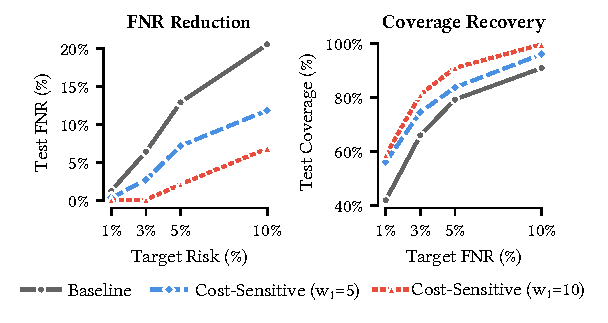
\includegraphics[width=\linewidth]{figures/Results_Comparison.pdf}
    \caption{Corresponding thresholds under different FNR targets.}
    \label{fig:risk_summary}
\end{figure}

Figure \ref{fig:risk_summary} compares the baseline and cost‑sensitive models. The left panel shows that standard risk control (Baseline, gray curve) yields relatively high FNR when calibrated only for target risk. By adding cost‑sensitive learning, the FNR is systematically reduced as the positive class weight increases to $w_1=5$ (blue) and $w_1=10$ (red). This confirms that penalizing false negatives during training drives the model toward a reliable decision-making mode.

The right panel illustrates the key strength of our approach. Under FNR‑centric calibration, the baseline model (gray) suffers severe coverage loss to meet strict safety targets (e.g., only $\sim40\%$ coverage at $1\%$ target FNR). In contrast, cost‑sensitive models recover substantial coverage. The $w_1=10$ model (red) maintains high coverage even at the $1\%$ FNR target, demonstrating that aligning the training objective (through cost weighting) with the calibration objective (FNR control) is an optimal strategy for deploying selective classification in safety‑critical clinical scenarios.


\subsection{External Validation}\label{S3-6}

We externally validated our models on the TRACERx 100 clinical cohort (\url{https://zenodo.org/records/10016027}), which comprises six histopathological subtypes (739 slides in total). For this binary classification task, we designated the micropapillary subtype as the positive class (149 samples) and the remaining five subtypes as the negative class (590 samples). We evaluated both the baseline models (Section \ref{S3-2}, Table \ref{tab:cv_results}) and the CSL+NP models (Section \ref{S3-4}, Table \ref{tab:csl_np_results}) on this external dataset, with results reported in Table \ref{tab1}.

\begin{table}[htbp]
    \centering
    \caption{The prediction performance of Baseline and NP with CSL.}
    \label{tab1}
    \resizebox{75mm}{!}{
    \begin{tabular}{ccccc}
        \toprule
        Strategy & ACC & AUC & FNR & FPR \\
        \midrule
        Baseline & 93.64\% & 90.64\% & 33.83\% & 3.19\% \\
        \midrule
        \multicolumn{5}{c}{Cost-Sensitive ($w_{1}=5$)} \\
        \midrule
        NP (1\%) & $35.49\%$ & $92.49\%$ & $0.67\%$ & $72.63\%$ \\
        NP (5\%) & $69.05\%$ & $92.49\%$ & $6.53\%$ & $34.05\%$ \\
        NP (10\%) & $79.41\%$ & $92.49\%$ & $12.00\%$ & $21.68\%$ \\
        \bottomrule
    \end{tabular}
    }
\end{table}

On the external dataset, the baseline achieved an accuracy of 93.64\% but incurred a high false negative rate (FNR) of 33.83\%. To address this, we applied cost-sensitive methods during training and NP methods during validation to control the FNR. With a target FNR of 5\%, our approach yielded an actual FNR of 6.53\% and an accuracy of 69.05\%. Compared to the baseline, this represents a 27.3 percentage point reduction in FNR at the cost of a 24.59 percentage point decrease in accuracy. 
\begin{table}[htbp]
    \centering
    \caption{The selective classification performance of external validation.}
    \label{tab2}
    \renewcommand\arraystretch{1.2} 
    \resizebox{85mm}{!}{
    \begin{tabular}{ccccc}
        \toprule
        Target Risk/FNR & Test Coverage & Test Risk & Test FNR & Test AUC \\
        \midrule
        \multicolumn{5}{c}{Case 3 ($w_{1}=5$, Risk control)} \\
        \midrule
        $1.00\%$ & $32.22\%$ & $2.07\%$ & $0.80\%$ & $98.82\%$ \\
        $5.00\%$ & $61.19\%$ & $4.87\%$ & $7.47\%$ & $97.23\%$ \\
        $10.00\%$ & $90.76\%$ & $9.27\%$ & $14.93\%$ & $95.53\%$ \\
        \midrule
        \multicolumn{5}{c}{Case 4 ($w_{1}=5$, FNR control)} \\
        \midrule
        $1.00\%$ & $41.14\%$ & $3.25\%$ & $1.87\%$ & $98.58\%$ \\
        $5.00\%$ & $56.70\%$ & $4.28\%$ & $3.20\%$ & $97.85\%$ \\
        $10.00\%$ & $84.22\%$ & $10.23\%$ & $10.67\%$ & $95.27\%$ \\
        \bottomrule
    \end{tabular}
    }
\end{table}

We further evaluated the selective inference framework on the external dataset and Table~\ref{tab2} summarizes the results. Under both risk control and FNR control, the framework achieved well calibrated performance on the external data, closely mirroring the behavior observed on our local validation set (Tables~\ref{tab:case3_results} and~\ref{tab:case4_results}). Overall, these results demonstrate that the framework maintains satisfactory predictive accuracy and selective classification performance on external data, consistent with its performance on local data.

\section{Conclusion}

In this work, we present a risk-controlled framework for MIP subtype detection in lung adenocarcinoma that systematically resolves the trade-off between diagnostic safety and throughput. Cost-sensitive learning reshapes the decision boundary by upweighting false-negative penalties, thereby boosting intrinsic model sensitivity prior to any threshold adjustment. Building on this shifted score distribution, Neyman--Pearson calibration translates the improved separability into a rigorous statistical guarantee that the false-negative rate remains below a clinically specified level, demonstrating that the two components are mutually reinforcing rather than independent. Selective classification further consolidates reliability by allowing the model to abstain on uncertain inputs, restricting automated decisions to a high-confidence subset while deferring ambiguous cases to pathologists. Together, these three phases achieve a principled balance between safety and efficiency, offering a deployable pathway toward trustworthy clinical decision support in high-stakes pathological diagnosis.

However, several issues merit further investigation. First, while the NP umbrella method can control the overall FNR at a specified level, which is an algorithm and data independent guarantee, it requires a separate set of positive validation samples. In clinical practice, positive samples are often the minority class, which can exacerbate training difficulty and compromise predictive accuracy. Second, although selective classification provides a theoretical lower bound on the risk–coverage tradeoff, controlling overall risk does not necessarily guarantee control of the FNR. Although cost-sensitive learning (Case 2 in Section \ref{sec:phase3_method}) empirically reduces the FNR, its theoretical assurance remains an open question for future work.


\section*{References}

\bibliographystyle{IEEEtran}
% Loading bibliography database
\bibliography{references}


\appendices

\section{Proof of Main Results}\label{S6}

\subsection{Proof of Theorem \ref{Th1}}\label{S6-1}

\begin{proof}
Let $Z_1, \dots, Z_{m_1}$ be the i.i.d. calibration positives with continuous CDF $F(t) = \mathbb{P}(Z \leq t)$. 
Define $U_i = F(Z_i)$. 
By the probability integral transform, $U_1, \dots, U_{m_1} \stackrel{\text{i.i.d.}}{\sim} \mathrm{Uniform}(0,1)$. 
Since $F$ is strictly increasing, the order statistics satisfy $F(\hat{p}_{(k)}) = U_{(k)}$, where $\hat{p}_{(k)}$ is the $k$-th smallest calibration score and $U_{(k)}$ the $k$-th uniform order statistic.  

Thus,
\[
\mathrm{FNR}(\hat{\tau}_{\alpha,\delta}) = F(\hat{p}_{(k)}) = U_{(k)}.
\]

The event $\{U_{(k)} > \alpha\}$ is equivalent to having fewer than $k$ uniform variables below $\alpha$. 
If $B \sim \mathrm{Binomial}(m_1, \alpha)$, then
\[
\mathbb{P}\bigl(U_{(k)} > \alpha\bigr) 
= \mathbb{P}(B \le k-1) 
= \sum_{j=0}^{k-1} \binom{m_1}{j} \alpha^j (1-\alpha)^{m_1-j}.
\]

Selecting $k$ such that this sum does not exceed $\delta$ gives
\[
\mathbb{P}\bigl(\mathrm{FNR}(\hat{\tau}_{\alpha,\delta}) > \alpha\bigr) = \mathbb{P}\bigl(U_{(k)} > \alpha\bigr) \le \delta.
\]
This bound holds for any scoring function because the reduction to uniform order statistics relies only on the i.i.d. calibration assumption and continuity of $F$, without dependence on the model class or complexity.
\end{proof}

\subsection{Proof of Theorem \ref{Th2}}\label{S6-2}

\begin{proof}
\textbf{Step 1: Risk Control ($R(f,g) \leq \epsilon$).}


Since the loss $\ell$ is bounded in $[0,1]$ and the accepted samples are independent Bernoulli random variables given $(f,g)$, we apply Hoeffding's inequality:
\[
\mathbb{P}\bigl(|\hat{R}_n(f,g) - R(f,g)| > t\bigr) \leq 2\exp\bigl(-2n_a t^2\bigr),
\]
where $n_a = \sum_{i=1}^n g(X_i)$ is the number of accepted samples.

We need to bound the deviation uniformly over all possible $(f,g)$, which are determined by the function class $\mathcal{F}$ and the acceptance region. A key observation is that each $(f,g)$ corresponds to an ``accept-error'' pattern: for each $X \in \mathcal{X}$, there are three states (accept and correct, accept and incorrect, reject), which can be encoded as a mapping $\mathcal{X} \to \{0,1,\bot\}$.
A counting argument shows that the number of possible $(f,g)$ patterns is at most:
\[
N \leq 3^{\min\{|\mathcal{F}|,|\mathcal{X}|\}} \leq 2^{(\ln 3 / \ln 2) \min\{|\mathcal{F}|,|\mathcal{X}|\}} \approx 2^{1.58 \min\{|\mathcal{F}|,|\mathcal{X}|\}}.
\]
Using a tighter bound where $(f,g)$ is determined by $(f, \Lambda)$ with $\Lambda \subseteq \mathcal{X}$ as the acceptance region, we apply the union bound:
\begin{align*}
    & \mathbb{P}\bigl(\exists (f,g) : |\hat{R}_n(f,g) - R(f,g)| > t\bigr) \\
    & \leq \sum_{(f,g)} \mathbb{P}\bigl(|\hat{R}_n(f,g) - R(f,g)| > t\bigr) \\
    & \leq N \cdot 2\exp\bigl(-2n_{a} t^2\bigr) \leq 2 \cdot 2^{1.58 \min\{|\mathcal{F}|,|\mathcal{X}|\}} \cdot \exp\bigl(-2n_{a} t^2\bigr),
\end{align*}

Setting this probability upper bound to $\delta/2$ and solving for $t$:
\[
\frac{\delta}{2} = 2 \cdot 2^{1.58\min\{|\mathcal{F}|,|\mathcal{X}|\}} \cdot \exp\bigl(-2n_{a} t^2\bigr)
\]
\[
t = \sqrt{\frac{1}{2n_{a}} \left( \ln 2 \cdot 1.58\min\{|\mathcal{F}|,|\mathcal{X}|\} + \ln \frac{4}{\delta} \right)}.
\]
Since the CSS selection ensures $\hat{R}_n(f,g) \leq \epsilon/2$ with probability at least $1-\delta/2$, we have:
\[
R(f,g) \leq \hat{R}_n(f,g) + t \leq \epsilon/2 + t.
\]


Setting $t = \epsilon/2$, we substitute into the probability bound:
\[
\frac{\delta}{2} = 2 \cdot 2^{1.58\min\{|\mathcal{F}|,|\mathcal{X}|\}} \cdot \exp\bigl(-2n_{a} (\epsilon/2)^2\bigr),
\]
which rearranges to:
\[
\epsilon = \sqrt{\frac{1}{n_{a}} \left( \ln 2 \cdot 3.16\min\{|\mathcal{F}|,|\mathcal{X}|\} + 2\ln \frac{4}{\delta} \right)}.
\]
As a result, with probability at least $1-\delta/2$, the selective classifier $(f,g)$ selected by CSS satisfies $R(f,g) \leq \epsilon$.

\textbf{Step 2: Coverage Control (Lower Bound on $\Phi(f,g)$).}

Given a risk tolerance $\epsilon$, we define the approximate function space:
\[
V_{\mathcal{F},S_n}^\epsilon = \bigl\{ f \in \mathcal{F} : \hat{R}_n(f) \leq \epsilon/2 \bigr\},
\]
where $\hat{R}_n(f)$ is the empirical risk of $f$ over the training set.
For a subset $G \subseteq V_{\mathcal{F},S_n}^\epsilon$, we define its \emph{$\epsilon$-uniform region}:
\[
\Lambda_G^\epsilon = \bigl\{X \in \mathcal{X} : \mathbb{P}_{f \in G}\bigl(\text{error at } X\bigr) \leq \epsilon \bigr\},
\]
meaning that the error rate of hypotheses in $G$ on $\Lambda_G^\epsilon$ does not exceed $\epsilon$.


Fix a subset $G$ and assume the measure of its $\epsilon$-uniform region is small: $P(\Lambda_G^\epsilon) \leq 1-\eta$.
If the CSS strategy selects a policy based on $G$ (i.e., the acceptance region is $\Lambda_G^\epsilon$), then:
\begin{itemize}
    \item All training points must lie within $\Lambda_G^\epsilon$ (otherwise there would be training errors).
    \item Alternatively, points lying outside $\Lambda_G^\epsilon$ must be classified correctly.
\end{itemize}
More precisely, if $G$ is selected as the ``base hypothesis set'', the errors in the training set must be tolerable.
Consider the event $E_G: G \subseteq V_{\mathcal{F},S_n}^\epsilon$ and the CSS strategy based on $G$ is selected. Then:
\[
\mathbb{P}(E_G) \leq (1-\eta+\epsilon)^m.
\]
This follows because for each point:
\begin{itemize}
    \item It lies outside $\Lambda_G^\epsilon$ with probability $\leq 1-\eta$.
    \item It may be misclassified outside $\Lambda_G^\epsilon$ with probability $\leq \epsilon$.
\end{itemize}


The number of possible subsets $G$ is of the order $2^{1.58\min\{|\mathcal{F}|,|\mathcal{X}|\}}$.
Applying the union bound:
\[
\mathbb{P}\bigl(\exists G : E_G\bigr) \leq 2^{1.58\min\{|\mathcal{F}|,|\mathcal{X}|\}} \cdot (1-\eta+\epsilon)^m.
\]
Using the inequality $1-\eta+\epsilon \leq \exp(-\eta+\epsilon)$, we obtain:
\[
\mathbb{P}\bigl(\exists G : E_G\bigr) \leq 2^{1.58\min\{|\mathcal{F}|,|\mathcal{X}|\}} \cdot \exp\bigl(-m(\eta-\epsilon)\bigr).
\]

Set the probability upper bound to $\delta/2$:
\[
\frac{\delta}{2} = 2^{1.58\min\{|\mathcal{F}|,|\mathcal{X}|\}} \cdot \exp\bigl(-m(\eta-\epsilon)\bigr).
\]
Solving for $\eta$:
\[
\eta - \epsilon = \frac{1}{m} \left( \ln 2 \cdot 1.58\min\{|\mathcal{F}|,|\mathcal{X}|\} + \ln \frac{2}{\delta} \right),
\]
\[
\eta = \epsilon + \frac{1}{m} \left( \ln 2 \cdot 1.58\min\{|\mathcal{F}|,|\mathcal{X}|\} + \ln \frac{2}{\delta} \right).
\]
Since the coverage $\Phi(f,g) \geq 1-\eta$, we conclude:
\[
\Phi(f,g) \geq 1 - \epsilon - \frac{1}{m} \left( \ln 2 \cdot 1.58\min\{|\mathcal{F}|,|\mathcal{X}|\} + \ln \frac{2}{\delta} \right).
\]
\end{proof}


\end{document}
